As we already showed, there was no way to get around at least adapting an existing routing engine. As Traveling Salesman is the one to use as a basis, our version of Traveling Salesman implementing the routing interface defined within the Kangaroo routing Framework is called \emph{MobileTSM}. The folling will summarize its structure, explain the most important changes in contrast to the original version of Traveling Salesman and give reasons for the adaptions.

\subsubsection{Major problems arising with decision for Traveling Salesman}

Coming up with the decision for using Traveling Salesman, there were several issues to work on:

\begin{enumerate}
	\item \textbf{Data storage}
	
		The data storage modules (data sets in Traveling Salesman's terminology) that come with the project can be considered unoptimized or even bad with respect to efficency and performance as needed for a mobile application. There are several different types of data set modules with different approaches of storing and organizing data.\newline
		
		Generally, but on Android's mobile platform in particular, there are two contradictory goals for the data storage architecture. Since Android restricts the heap space for an application to (at this time) 16 megabytes, the map area that can be cached in memory, is limited to several square kilometers, depending of course on data density. Thus one is forced to filter map elements before loading into memory.
		As not only memory is expensive, but also data access to a flash card or a database, a compromise has to be found between loading the whole map into memory and accessing the persistent map database for every single element requested by the routing engine.
				
	\item \textbf{Routing data}
	
		By default, Traveling Salesman performs every routing operation on the original set of data not dropping elements that do not affect the result of the operation. An example for elements of this type are nodes, that geographically shape the curvature of a street but do not introduce a junction. A node of this type will be called \emph{intermediate way node} and is dispensable for routing operations unless it is the nearest node to the starting or destination point of a route. Any other way node will be called \emph{essential way node}.\newline
		
		Both memory space occupied by the map and time consumption of a routing operation can be reduced by ignoring intermediate way nodes. Nethertheless one cannot dispense with intermediate way nodes close to starting and destination point. This implies an individual routing data set for every routing operation. At first sight this induviduality runs contrary to Traveling Salesman's architecture when aiming at keeping compatibility. We will show a way to individualize routing data while maintaining full compatibility.
											
	\item \textbf{Searching algorithm}
	
		When given two pairs of geographical coordinates and an order to find a route between these two, one has to find the nearest street nodes to starting and destination locations prior to the actual routing operation. This is because non-trivial routing operations can only be performed on a routing graph between vertices. Thus one has to translate from a geographical location to the vertex (node) that best matches it. This can be considered the street node with minimal distance to the given location.\newline
				
		A naive ansatz to finding the nearest street node 	to a geoprahical location would be to iterate over all street nodes, calculate the distance between the location and each street node and select the one with minimal distance. Exactly this is done by Traveling Salesman resulting in an extremly time consuming routing process.\newline

\end{enumerate}


\subsubsection{Approaches for major problems arising with decision for Traveling Salesman}
\label{sec:routing_mobiletsm_approaches}

As just explained in the previous section, three main issues have to be handled: reduce and individualize routing data while maintaining compatibility to Traveling Salesman, find an efficient data storage architecture and improve the search algorithm for nearest nodes. The next sections will outline the abstract framework designed to approach these problems.

\begin{enumerate}
	\item \textbf{Reducing and individualizing of routing data}

As routing data should be reduced and individualized before it is used by any Traveling Salesman module, a preprocessor has to be inserted. The basic idea to do this is to introduce a module, an abstract Java class named \texttt{MobileDataSetProvider}, that can be queried for a specialized set of routing data which is compatible with Traveling Salesman and optimized for an individual routing operation.\newline

Basically an individual routing data set has to contain all essential way nodes and intermediate way nodes of the start and destination ways. If start and destination nodes are essential way nodes itself, it can completly abstain from intermediate way nodes.\newline

\begin{figure}[h!]
	\centering
	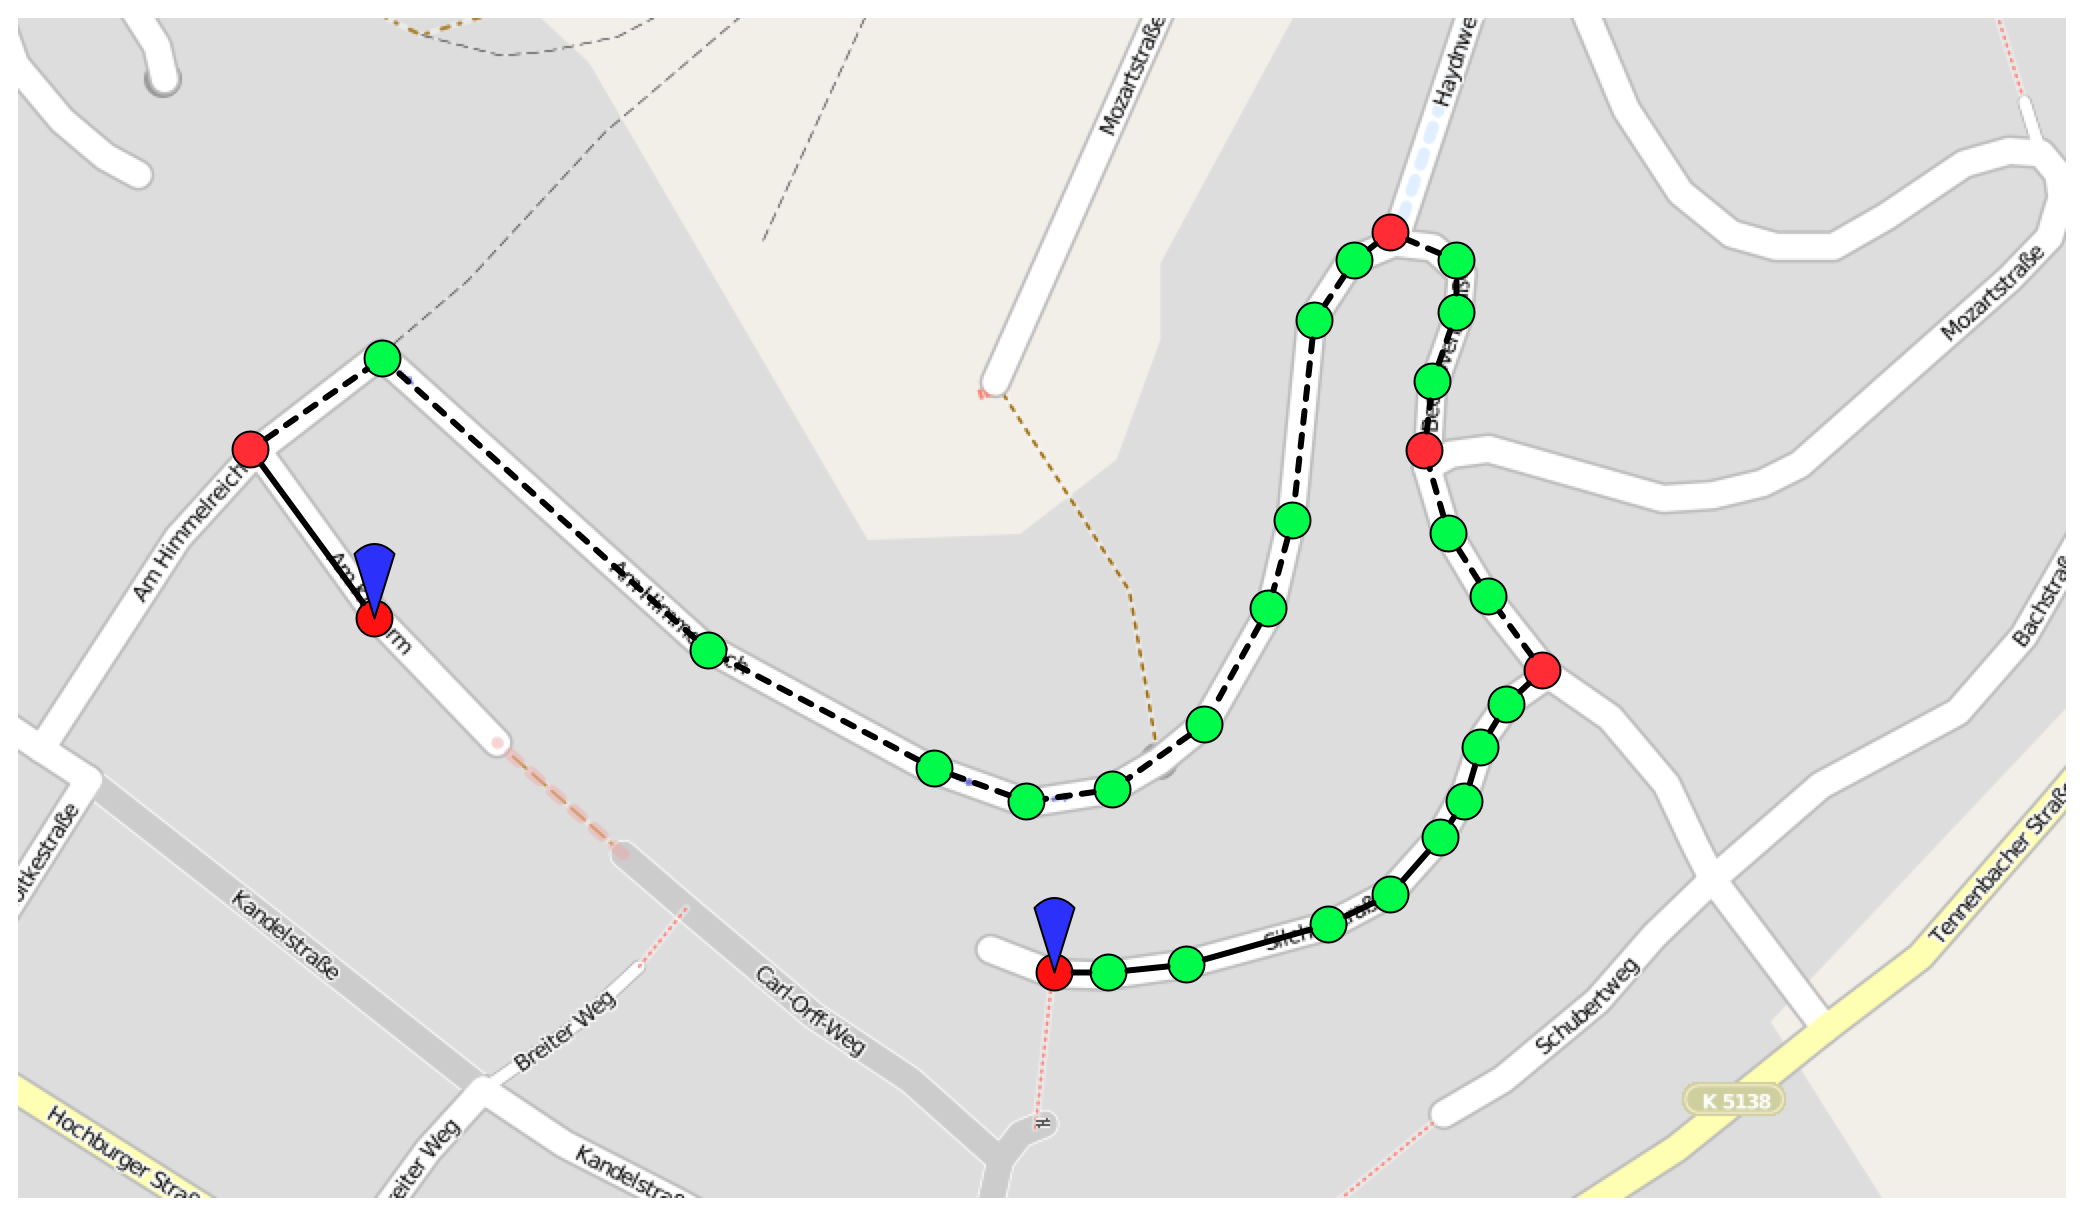
\includegraphics[width=12cm]{pics/routing_data.png}
	\caption{A route including intermediate way nodes: The blue markers define start and destination of the route, red points define essential street nodes and green points define intermediate way nodes. The corresponding routing graph constains much more elements than needed for the routing operation.}
	\label{fig:routing_data}
\end{figure}

\begin{figure}[h!]
	\centering
	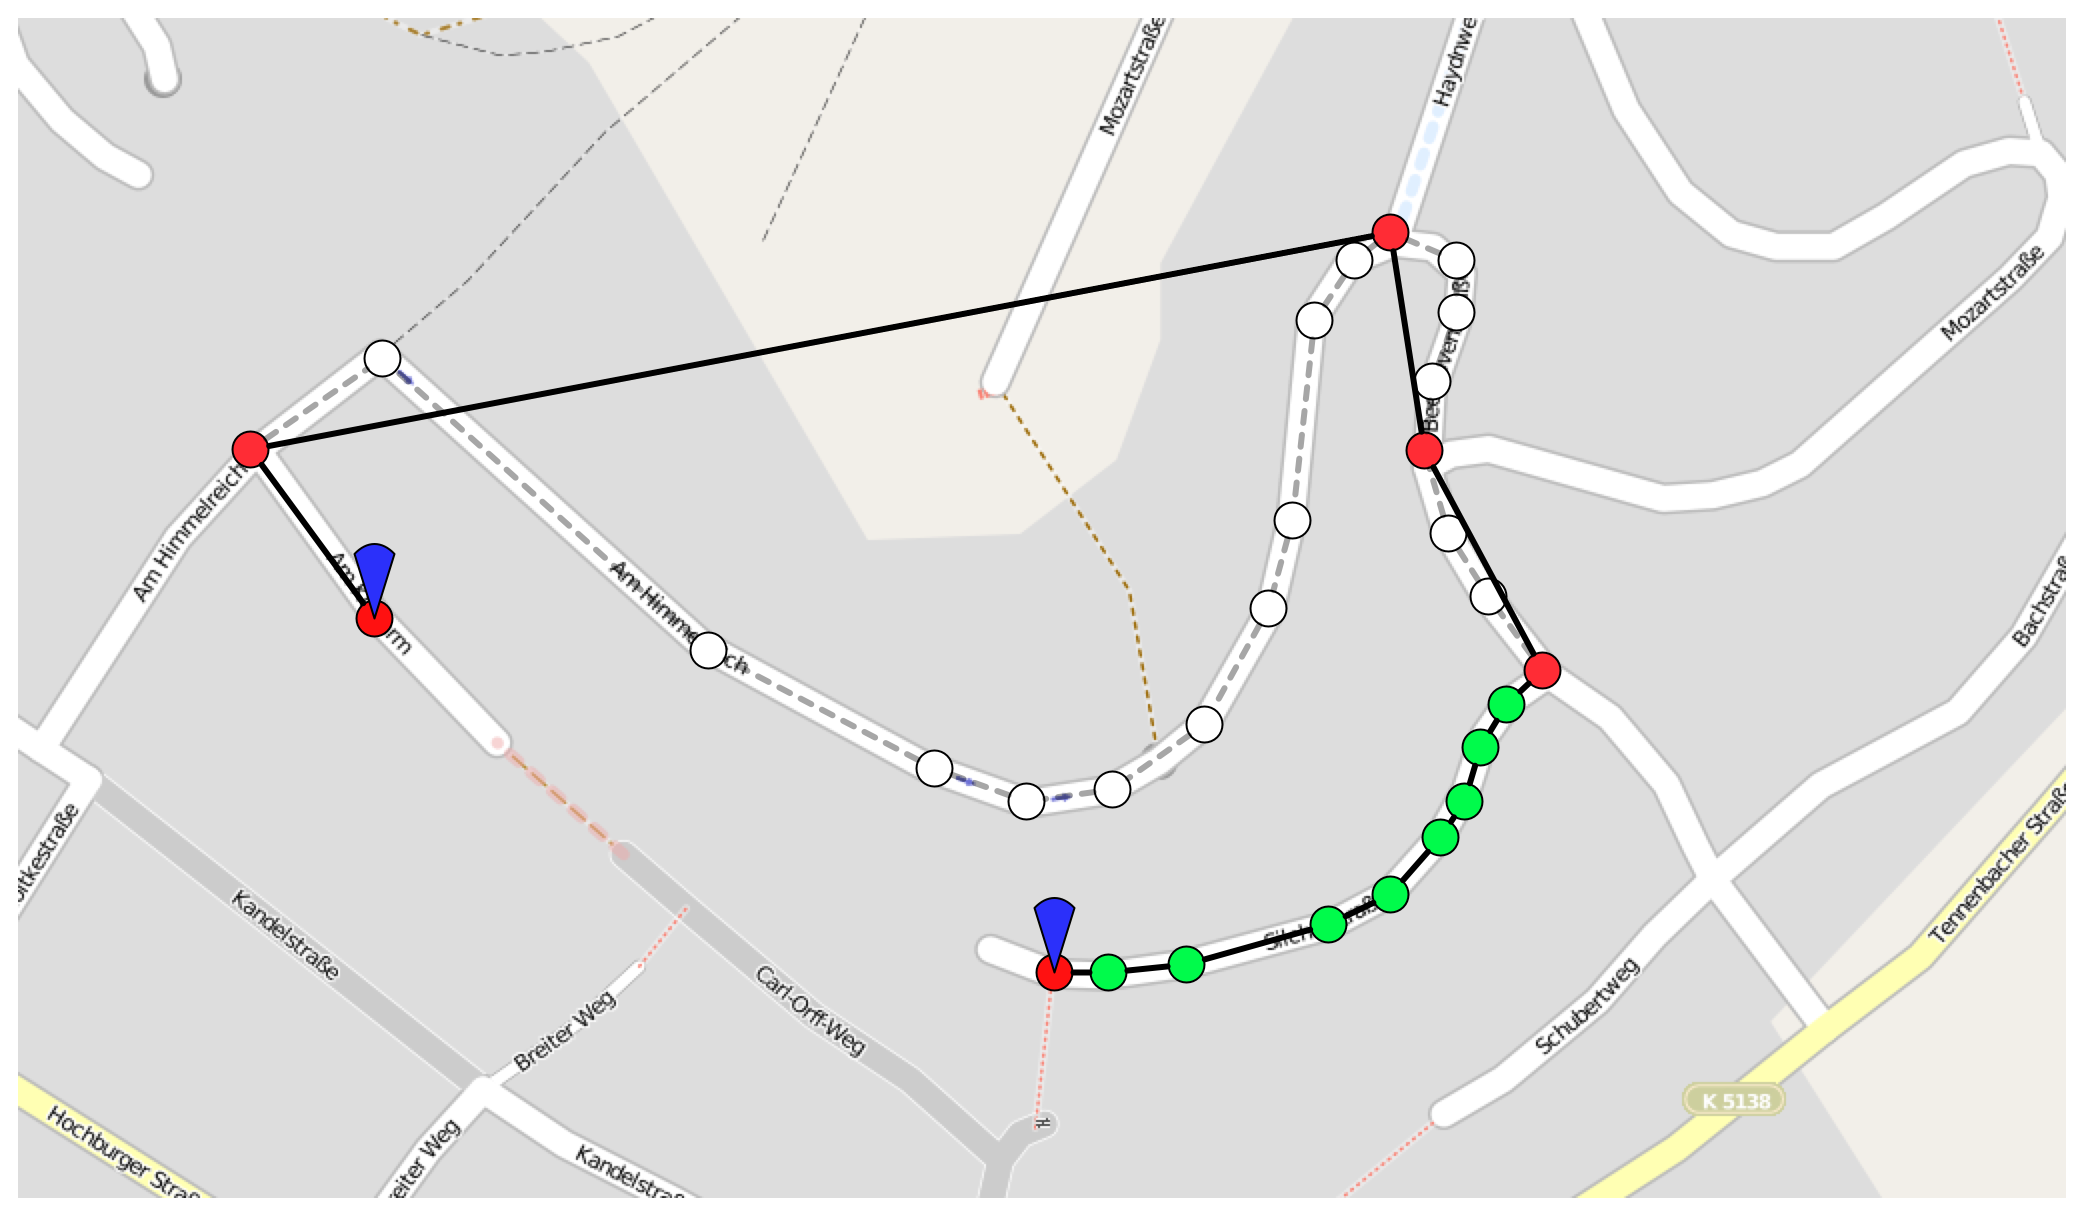
\includegraphics[width=12cm]{pics/routing_data_2.png}
	\caption{The same route like the one in \ref{fig:routing_data} but without intermediate way nodes. Routing on this individually reduced routing graph will yield the same shortest path (assuming revision of distance errors, cf. next clauses).}
	\label{fig:routing_data_2}
\end{figure}

Internally, all essential street nodes and single intermediate way nodes requested by a routing operation are cached in memory. The individualized data set simply maps from queries performed on it to these caches. As it externally behaves like a Traveling Salesman data set, any Traveling Salesman router may then be called with a reference to this individual data set. Anyhow, a router can perform another routing operation with different parameters on the same data set, but since the majority of intermediate way nodes will not be included in the data set, it will probably not find the best route or might even fail.\newline

One can also think of adding functionality to recycle an individualized data set. Instead of creating a new one for each routing operation, an old data set may be updated to be as qualified as if it was created specifically for the new parameters. One may be tempted to believe this is the only way to significantly gain time resources, but we will show that in fact our implementation exploits major improvements without this feature.\newline

When dropping intermediate way nodes one has to be aware that Traveling Salesman calculates the distance of a route by hopping from node to node summing up their linear distances. To revise the error induced by missing intermediate way nodes, an extra property has to be added to ways giving the real distance between two way nodes. That is the main reason for introducing a derivate of Osmosis' \texttt{Way} class, called \texttt{MobileWay} and  a derivate of Traveling Salesman's \texttt{WayNode} class, called \texttt{MobileWayNode}

	\item \textbf{Data storage architecture}

The data set provider itself reads data from a suitable data source (for example from database or a file stream). Since even individualized data sets will have a large intersection, data is cached in memory to a great extent to avoid reloading of data already read due to a prior routing query.\newline

As an abstraction of the data access to a routing data sources, a Java interface (called \texttt{RoutingDataAdapter}) is introduced. It provides methods to read map elements from a given data source.\newline

To become more tangible, the abstract \texttt{RoutingDBAdapter} class as a derivation of the \texttt{RoutingDataAdapter} class will be used to access a database as source for routing data. A further derivation of the \texttt{RoutingDBAdapter} class, called \texttt{RoutingAndroidSQLiteAdapter}, finally implements the access to the Android specific SQLite database. For a describtion of this database structure and its creation, look at section \ref{sub:routing_database}\newline

With this type of abstraction it is still possible to exchange the SQLite database by another type of database or even not to use any database system at all but for example a proprietary file format. Nevertheless the SQLite database of Android seemed to be the most promising one, since one can expect of it to be highly optimized while maintaining a great degree of flexibility. In deed, any of our tests gave reason to be in doubt about this expectation.

	\item \textbf{Search algorithm for nearest nodes}

As already demonstrated, the search for the nearest street node is an integral part of a routing operation. Without any assumption about the chronological and geographical pattern of routing operations that will be performed, one has to improve the data structure storing the nodes to be qualified for fast random access. Anyhow, one can think of another way to speed up the search when analyzing the average use.\newline

\begin{figure}[h!]
	\centering
	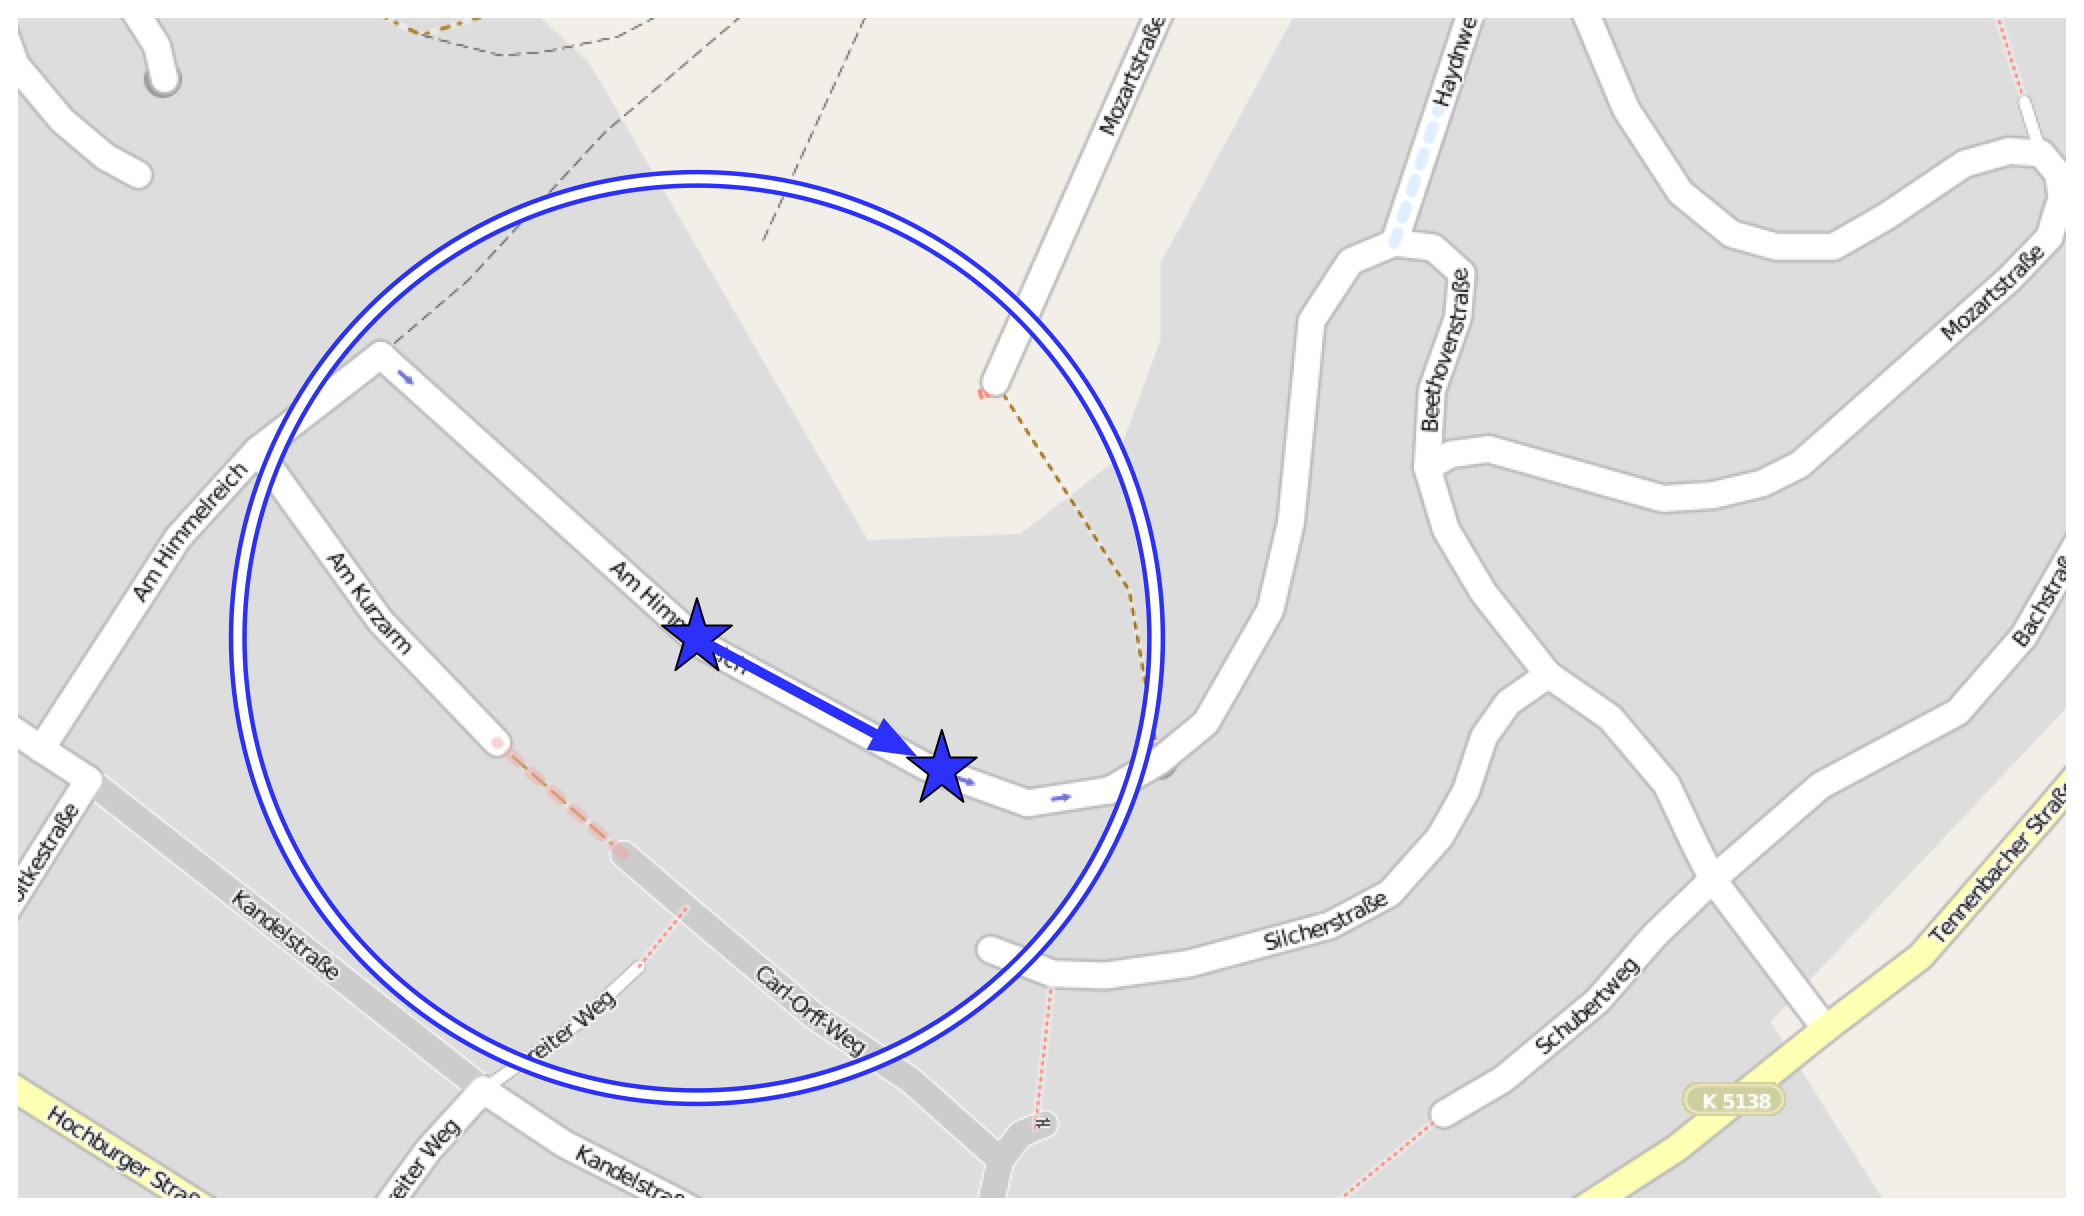
\includegraphics[width=12cm]{pics/nearest_node_cache.png}
	\caption{Caching of nearest street nodes: The first query is used to cache street nodes within a specified radius of the query center. Under appropriate conditions the next query does not have to access the database but only the cache.}
	\label{fig:nearest_node_cache}
\end{figure}

Besides routing operations performed in advance\footnote{routing operations that are only based on calendar items and that are independent from current position}, the routing engine will also be triggered with routing operations using the current position. Since the current position is likely to change slowly in contrast to a random access, performance may be improved by caching street nodes inside a given radius around the last query. Figure \ref{fig:nearest_node_cache} gives a graphical representation.


	\item \textbf{Caching of calculated routes}
	
		Routing operations may and will in principle have random parameters based on calendar items and the current position. Anyhow, it is highly probable that antecedent routing operations recur after a while. If one can make sure that the operation's parameter exactly match, there is no sense to recalculate the route\footnote{Note that this assumes restriction to static routing data}. It may rather reuse the result of the respecting routing operation.\newline
		
		\emph{MobileTSM} introduces a routing cache that efficiently stores results of antecedent routing operations by using a kind of double hashing. When triggering a new routing operation, the routing cache will be checked in advance and only if there is no matching result of an antecedent routing operation, the routing engine will actually perform the routing operation.


\end{enumerate}

\subsubsection{Structure of MobileTSM}
\label{subsubsec:routing_mobiletsm_structure}

\begin{itemize}
		
	\item Class \texttt{MobileTSMRoutingEngine}
	
		The class \texttt{MobileRoutingEngine} is the \emph{MobileTSM} implementation of the \texttt{RoutingEngine} introduced with the Kangaroo routing framework. It provides the routing services used by the main application, including the previously explained routing cache.
		
	\item Class \texttt{Vehicle}
	
		The abstract class \text{Vehicle} implements Traveling Salesman's \texttt{IVehicle} interface which is thought to define and constrain the usage of streets and ways. These constraints will be considered by the routing engine when being passed as a parameter of a routing operation. It also adds the possibility to specify a maximum speed. The routing engine will account for this maximum speed when calculation the duration of travel of a route.\newline
		
		There a several derivates of this class defining different types of vehicles, including appropriate maximum speeds (for example \texttt{AllStreetVehicle}).
	
	\item Class \texttt{MobileTSMRouteParameter}
	
		This class is a direct derivate of the abstract \texttt{RouteParameter} class. It includes the algorithm to calculate the duration of travel of a Traveling Salesman route based upon the route and the used vehicle.

	\item Class \texttt{POICode}

		This class is used to represent one type of a Point Of Interest. It also provides a mapping between possible tags of Openstreetmap and an unique integer value.
	
	\item Classes \texttt{MobileNode}, \texttt{MobileWay}, \texttt{MobileWayNode} 
	
		The need and sense of introducing the derivated classes \texttt{MobileWay} and \texttt{MobileWayNode} was already pointed out and won't be repeated. The derivated class \texttt{MobileNode} is introduced to be able to associate a reference to a nearest street node and a Point Of Interest (represented by an instance of \texttt{POICode}) to the node.

	\item Class \texttt{MobileMultiTargetDijkstraRouter}

		As already stated in chapter \ref{sub:routing_tsm}, Traveling Salesman's router class \texttt{MultiTargetDijkstraRouter} seems to be implemented incorrectly. It actually is supposed to be a Dijkstra algorithm extended to an A*-algorithm. This extension is characterized by the use of a heuristic for determining the next node to visit. In Traveling Salesman's original implementation, this heuristic and the data structure holding the nodes to visit is not realized correctly, often yielding not the shortest path as a result. These implementation errors are fixed in the \texttt{MobileMultiTargetDijkstraRouter} router class.
	
	\item Class \texttt{MobileRoutingMetric}
	
		As explained above, dropping intermediate way nodes results in the need for an adapted measure of distances on a way. Since the routing metric (\texttt{IRoutingMetric}) is a self-contained module, it can easily exchanged by a metric (\texttt{MobileRoutingMetric}) using the corrected distance measure.\newline
		
		Like Traveling Salesman's default implementation \texttt{ShortestRouteMetric} also the new implementation does not privilege any type of street. The undesirable effect of finding the shortest but not definitely the fastest route still persists and may be abolished as part of a future extension.

\end{itemize}



